\documentclass[reqno,12pt,oneside]{report} % right-side equation numbering, 12 point font, print one-sided
%\documentclass[reqno,12pt,twoside,openright]{report} % right-side equation numbering, 12 point font, print two-sided, Chapters start on odd pages. Rackham only accepts one-sided, so this is for personal printings.

\usepackage{rac}         % Use Rackham thesis style file
%\usepackage{aas_macros}  % To allow the reading of ADS journal references in the bibliography
\usepackage[intlimits]{amsmath} % Puts the limits of integrals on top and bottom
\usepackage{amsxtra}     % Use various AMS packages

\usepackage{amsthm}
\usepackage{amssymb}
\usepackage{graphicx}    % Add some packages for figures. Read epslatex.pdf on ctan.tug.org

\usepackage{rotating}
\usepackage{color}
\usepackage{xspace}
\usepackage{mdframed}
\usepackage{epsfig}
\usepackage{subfigure}   % To make subfigures. Read subfigure.pdf on ctan.tug.org
\usepackage{multirow}

\usepackage{verbatim}
\usepackage[numbers]{natbib}      % Allows you to use BibTeX
\usepackage{acronym} % For the List of Abbreviations. Read acronym.pdf on ctan.tug.org
\usepackage{booktabs}% http://ctan.org/pkg/booktabs
\newcommand{\tabitem}{~~\llap{\textbullet}~~}
\usepackage{indentfirst}
\usepackage{enumitem}
\usepackage{setspace}
\usepackage[T1]{fontenc}
\usepackage[utf8]{inputenc}
%\usepackage[options ]{algorithm2e}
\usepackage{algpseudocode}
\usepackage{ifthen}
%\usepackage{mathptmx} 
%\usepackage[acronym]{glossaries}
%\usepackage{nomencl}
%\usepackage[noend]{algpseudocode}
%\usepackage[linesnumbered,ruled,vlined]{algorithm2e}

\usepackage[intoc]{nomencl}
\usepackage{tikz}
\usetikzlibrary{shapes.geometric, arrows}

\usepackage{url}
%\usepackage{breakurl}
%\usepackage[breaklinks]{hyperref}
% \usepackage{hyperref}
 
 \usepackage{algorithm,algpseudocode}


%\usepackage[latin1]{inputenc}
%\usetikzlibrary{shapes,arrows}
\tikzstyle{startstop} = [rectangle, rounded corners, minimum width=3cm, minimum height=1cm,text centered, draw=black, fill=red!30]
\tikzstyle{io} = [trapezium, trapezium left angle=70, trapezium right angle=110, minimum width=3cm, minimum height=1cm, text centered, draw=black, fill=blue!30]
\tikzstyle{process} = [rectangle, minimum width=3cm, minimum height=1cm, text centered, draw=black, fill=orange!30]
\tikzstyle{decision} = [diamond, minimum width=3cm, minimum height=1cm, text centered, draw=black, fill=green!30]
\tikzstyle{arrow} = [thick,->,>=stealth]

%%%<


\usepackage[nottoc,notlof,notlot]{tocbibind}
\renewcommand\bibname{References}

\makenomenclature
%\makenomenclature
  % Allows you to specify the line spacing
%\doublespacing
\onehalfspacing %for 1.5 spacing, %\doublespacing for 2.0 spacing.
\newcommand{\sun}{\ensuremath{\odot}} % sun symbol is \sun
%%%%%%%%%%%%%%%%%%%%%%%%%%%%%%%%%%%%%%%%%%%%%%%%%%%%%%%%%%%%%%%%%%%%%%%%%%%%%%%

% Various theorem environments. All of the following have the same numbering
% system as theorem.

\theoremstyle{plain}
\newtheorem{theorem}{Theorem}
\newtheorem{prop}[theorem]{Proposition}
\newtheorem{corollary}[theorem]{Corollary}
\newtheorem{lemma}[theorem]{Lemma}
\newtheorem{question}[theorem]{Question}
\newtheorem{conjecture}[theorem]{Conjecture}
\newtheorem{assumption}[theorem]{Assumption}

\theoremstyle{definition}
\newtheorem{definition}[theorem]{Definition}
\newtheorem{notation}[theorem]{Notation}
\newtheorem{condition}[theorem]{Condition}
\newtheorem{example}[theorem]{Example}
\newtheorem{introduction}[theorem]{Introduction}

\theoremstyle{remark}
\newtheorem{remark}[theorem]{Remark}
%%%%%%%%%%%%%%%%%%%%%%%%%%%%%%%%%%%%%%%%%%%%%%%%%%%%%%%%%%%%%%%%%%%%%%%%%%%%%%%

\numberwithin{theorem}{chapter}     % Numbers theorems "x.y" where x
                                    % is the section number, y is the
                                    % theorem number

%\renewcommand{\thetheorem}{\arabic{chapter}.\arabic{theorem}}

%\makeatletter                      % This sequence of commands will
%\let\c@equation\c@theorem          % incorporate equation numbering
%\makeatother                       % into the theorem numbering scheme

%\renewcommand{\theenumi}{(\roman{enumi})}

%%%%%%%%%%%%%%%%%%%%%%%%%%%%%%%%%%%%%%%%%%%%%%%%%%%%%%%%%%%%%%%%%%%%%%%%%%%%%%

% If printing two-sided, this makes sure that any blank page at the
% end of a chapter will not have a page number.
\makeatletter
\def\cleardoublepage{\clearpage\if@twoside \ifodd\c@page\else
\hbox{}
\thispagestyle{empty}
\newpage
\if@twocolumn\hbox{}\newpage\fi\fi\fi}
\makeatother

%%%%%%%%%%%%%%%%%%%%%%%%%%%%%%%%%%%%%%%%%%%%%%%%%%%%%%%%%%%%%%%%%%%%%%%%%%%%%%

%This command creates a box marked ``To Do'' around text.
%To use type \todo{  insert text here  }.

\newcommand{\todo}[1]{\vspace{5 mm}\par \noindent
\marginpar{\textsc{To Do}}
\framebox{\begin{minipage}[c]{0.95 \textwidth}
\tt\begin{center} #1 \end{center}\end{minipage}}\vspace{5 mm}\par}



\begin{document}
%\bibliographystyle{ieeetr}
%\bibliographystyle{plain}    % Set the bibliography style. agu04, plain, alpha, etc.
% Title page as required by Rackham dissertation guidelines
\titlepage{Co-operative Society And Loan Management System}{ 222149}{Professional Masters in Information Technology}
{Information Technology}{December 2023}
{Dr. M Shamim Kaiser, Professor}

% Begin the front matter as required by Rackham dissertation guidelines
\initializefrontsections

% Optional Frontispiece
%\frontispiece{\includegraphics[width=6in]{Intro/Happy} Find a cool picture to go here.}

% Optional, but recommended, Copyright page
%\copyrightpage{Your Name}

% Page numbering. If you don't include a frontispiece or copyright page, you'll need to change this for two-sided printing.
\makeatletter
\if@twoside \setcounter{page}{4} \else \setcounter{page}{1} \fi
\makeatother

% Optional Dedication page
%\dedicationpage{To Our Beloved Parents}


%Optional declaration page
\startdeclarationpage
I hereby declare that this thesis is based on the results found by ourselves. Materials
of work found by other researcher are mentioned by reference. This thesis, neither in
whole nor in part, has been previously submitted for any degree.

\vspace{1in}


\noindent   \rule{3.5cm}{1pt} \\
   Roll:152395 \\


\label{declaration}


%Optional Certificate page
\startcertificatepage
The project titled “Co-operative Society And Loan Management System” submitted by Md. Hasibuzzaman, ID: 222149, Session: Summer-2022, has been accepted as satisfactory in partial fulfillment of the requirement for the degree of Professional Masters in Information Technology on the 3rd of January 2023.

%\bigskip

\bigskip
\bigskip
\bigskip

\noindent \begin{tabular}{l}

  % after \\: \hline or \cline{col1-col2} \cline{col3-col4} ...
  \rule{4cm}{1pt} \\
  Dr. M. Shamim Kaiser\\ % replace it
  Supervisor\\

\end{tabular}


%Accepted and approved in partial fulfilment of the requirement for the degree Professional Master in Information Technology.


\begin{center}
   \textbf{BOARD OF EXAMINERS}
\end{center}
\noindent \begin{tabular}{lp{1cm}r}
\centering
  % after \\: \hline or \cline{col1-col2} \cline{col3-col4} ...
  \rule{4cm}{1pt}&\\
     Dr. Mohammad Abu Yousuf  &&Coordinator  \\
     Professor, IIT, JU  & & PMIT Coordination Committee  \\
     & &  \\
     \rule{4cm}{1pt}&\\
    Dr. M. Shamim Kaiser  & &Member, PMIT Coordination Committee   \\
     Professor, IIT, JU  & &\& Director, IIT\\
    & &  \\
     \rule{4cm}{1pt}&\\
     Dr. Shamim Al Mamun & &Member  \\
      Associate Professor, IIT, JU  & &PMIT Coordination Committee  \\
     &  \\
     \rule{4cm}{1pt}&\\
     Dr. Mohammad Shahidul Islam   & &Member  \\
      Associate Professor, IIT, JU  & &PMIT Coordination Committee  \\
      &  \\
     \rule{4cm}{1pt}&\\
     Dr. Md. Sazzadur Rahman  & &Member  \\
      Associate Professor, IIT, JU  & &PMIT Coordination Committee  \\
     
  %\rule{4cm}{1pt} & \rule{4cm}{1pt} & \rule{4cm}{1pt}\\
   

\end{tabular}


%\noindent \begin{tabular}{p{5cm}p{4cm}p{5cm}}
%\centering
  % after \\: \hline or \cline{col1-col2} %\cline{col3-col4} ...
   %  &  &   \\
    % &  &   \\
     %&  &   \\
  %\rule{4cm}{1pt} &  & \rule{3.5cm}{1pt}\\
  %Jesmin Akhter &   &K M Akkas Ali\\
  %Chairman &   &Member\\
   %  &  &   \\
    % &  &   \\
  %\rule{3.5cm}{1pt}& & \rule{3.5cm}{1pt}\\
   %Shamim Al Mamun&   &Prof. Dr. M. A. Mottalib \\
  %Member &   &Member (External) \\
%\end{tabular}


\label{Certificate}



% Optional Acknowledgements page
\startacknowledgementspage
We feel pleased to have the opportunity of expressing our heartfelt thanks and gratitude to those who all rendered their cooperation in making this report.








This thesis is performed under the supervision of Dr. M. Shamim Kaiser, Associate professor, Institute of Information Technology (IIT), Jahangirnagar University, Savar, Dhaka. During the work, he has supplied us a number of books, journals, and materials related to the present investigation. Without his help, kind support and generous time spans he has given, we could not perform the project work successfully in due time. First and foremost, we wish to acknowledge our profound and sincere gratitude to him for his guidance, valuable suggestions, encouragement and cordial cooperation.

We express our utmost gratitude to Dr. M Mesbahuddin Sarker, Director, IIT, Jahangirnagar University, Savar, Dhaka, for his valuable advice that have encouraged us to complete the work within the time frame. Moreover, we would also like to
thank the other faculty members of IIT who have helped us directly or indirectly by providing their valuable support in completing this work.

We express our gratitude to all other sources from where we have found help. We are indebted to those who have helped us directly or indirectly in completing this work.

Last but not least, we would like to thank all the staff of IIT, Jahangirnagar University and our friends who have helped us by giving their encouragement and cooperation throughout the work.
\label{Acknowledgements}

%Optional Abstract page
\startabstractpage
The Co-operative Society Management System is a comprehensive software solution created to streamline and automate the functions of Co-operative societies under the Bangladesh Rural Development Co-operative Division authority. This summary offers insights into its main features and advantages.

Co-operative societies are pivotal in sectors like agriculture, finance, and housing, fostering collaboration among members and fostering economic development. Yet, the management of administrative tasks and financial transactions within these societies can be intricate and time-intensive. The Co-operative Society Management System seeks to simplify these processes by providing an efficient and user-friendly platform.






\vspace{8pt}
\textbf{Keywords:} Coop, Co-operative Society Management System, Socity Management System, cooperative and loan Management System and Samity Management System.

\label{Abstract}




% List of Abbreviation

\listofabbreviations % Optional. Abbreviations should be stored in a file named abbr.tex
% Optional in-dissertation Abstract Page
%\startabstractpage
%{The Title of Your Dissertation}{Your Name}{Chair: Albert Einstein}
%The Co-operative Society Management System is a comprehensive software solution created to streamline and automate the functions of Co-operative societies under the Bangladesh Rural Development Co-operative Division authority. This summary offers insights into its main features and advantages.

Co-operative societies are pivotal in sectors like agriculture, finance, and housing, fostering collaboration among members and fostering economic development. Yet, the management of administrative tasks and financial transactions within these societies can be intricate and time-intensive. The Co-operative Society Management System seeks to simplify these processes by providing an efficient and user-friendly platform.






\vspace{8pt}
\textbf{Keywords:} Coop, Co-operative Society Management System, Socity Management System, cooperative and loan Management System and Samity Management System.

%\label{Abstract}

\section*{
\begin{center}
  LIST OF ABBREVIATIONS
\end{center}
}

\begin{tabular}{p{2.5cm}p{10cm}}
%\textbf{\symbab}  & \symbac\\
\textbf{IIT}  & Institute of Information Technology\\
\textbf{JU}  & Jahangirnagar University \\
\textbf{IIT}  & Institute of Information Technology \\
\textbf{IIT}  & Institute of Information Technology \\ 
% double back slash refers to newline
\textbf{QoS}  & Quality of Service \\

\end{tabular}



% List of Notatoin
\listofnotations
\section*{
\begin{center}
 LIST OF NOTATIONS
\end{center}
}


\begin{tabular}{p{2.5cm}p{10cm}}
%\textbf{\symbab}  & \symbac\\
$\alpha$  & Define alpha\\
$\max$  & maximum\\
$\cos{\theta}$ & maximum\\
$x$ & maximum\\ % for equation mode use $$; & next column

\end{tabular}

%\input{Preface}
%\label{Preface}
% Table of contents, list of figures, etc.
\listoffigures   % Required if there is more than one figure
\listoftables        % Required if there is more than one table
\tableofcontents     % Required

%\startprefacepage
\printnomenclature[1.5cm]

%%%%%%%%%%%%%%%%%%%\printnomenclature
%\clearpage



%\renewcommand{\arraystretch}{1.70}
%\begin{tabular}{p{2.5cm}p{10cm}}
%\centering
  %\rule{3.5cm}{1pt} & \rule{3.5cm}{1pt} & \rule{3.5cm}{1pt}\\
%  $\alpha$ & Define Alpha\\
%$\symba $ & \symbb\\
%$\symbc $ & \symbd\\
%$\symbe $ & \symbf\\
%$\symbg $ & \symbh\\
%$\symbi $ & \symbj\\
%$\symbk $ & \symbl\\
%$\symbm $ & \symbn\\
%$\symbo $ & \symbp\\
%$\symbq $ & \symbr\\
%$\symbs $ & \symbt\\
%$\symbu $ & \symbv\\
%$\symbw $ & \symbx\\
%\end{tabular}
%\newpage
%\begin{tabular}{p{2.5cm}p{10cm}}









%\listofmaps          % Required if there is more than one map
%\listofappendices    % Required if there is more than one appendix
%%%%--------------------------------------------------------------------------------
\startthechapters
% The individual files for each of the chapters are put here.
% Save each chapter of your thesis to a seperate tex file
% and then use the \input command to include this file in your
% thesis.  For instance you can save a file to "intro.tex" and
% then type \input{intro}.

 %\chapter{Introduction}
 \label{chap:Intro}
 

\chapter{Introduction}

%\label{chap:GettingStarted}
\section{Overview}
The introduction of a Co-operative Society Management System marks a significant leap
in the efficient and organized management of Co-operative societies. Co-operative
societies play a vital role in various sectors, including agriculture, finance, and housing,
by fostering collaboration among members and promoting economic development.
However, managing the diverse functions and operations of these societies can be
complex and demanding. This introduction provides an overview of the purpose, features,
and benefits of such a system.

\subsection{Purpose}
The Co-operative Society Management System is meticulously crafted to cater to the distinctive needs and challenges encountered by Co-operative societies. Its core objective is to simplify and automate the administrative, financial, and member-centric processes within a Cooperative society. Through this, the system aims to elevate efficiency, transparency, and overall performance, providing a comprehensive solution tailored to the intricate requirements of Co-operative societies.

% \section{Motivation}

% \subsection{Image Processing}



\section{The History of Co-operative Societies in Bangladesh}

The concept of Co-operative societies has a deep-rooted history in Bangladesh, dating back to the pre-independence period and gaining significant momentum in the post-independence era. Here's a brief background on Co-operative societies in Bangladesh:

\subsection{Pre-independence Period}

Co-operative societies in what is now Bangladesh can trace their origins to the British colonial period. During this time, Co-operative movements began to take shape, primarily in rural areas. These early Co-operatives aimed to address the economic challenges faced by farmers and rural communities. However, the concept remained somewhat limited in scope.

\subsection{Post-independence Era}

After gaining independence from Pakistan in 1971, Bangladesh faced numerous socio-economic challenges. Co-operatives were seen as a means to empower rural communities, alleviate poverty, and promote economic development. The government of Bangladesh began to actively promote and support Co-operative initiatives as part of its socioeconomic development strategy.

Co-operative societies in Bangladesh have a diverse history and have played a significant role in addressing rural and urban development challenges. With ongoing efforts to overcome challenges and promote transparency, Co-operatives continue to be a valuable instrument for socio-economic development and poverty reduction in the country.



\section{Aims of Co-operative Societies in Bangladesh}

The aims of Co-operative societies in Bangladesh are multifaceted and are aligned with socio-economic development, poverty reduction, and the empowerment of various segments of society. Here are the primary aims of Co-operative societies in Bangladesh:

\begin{enumerate}
    \item \textbf{Poverty Alleviation}
    \item \textbf{Rural Development}
    \item \textbf{Agricultural Advancement}
    \item \textbf{Financial Inclusion}
    \item \textbf{Empowerment of Women}
    \item \textbf{Housing and Urban Development}
    \item \textbf{Entrepreneurship Development}
    \item \textbf{Social Welfare}
    \item \textbf{Community Building}
    \item \textbf{Good Governance}
\end{enumerate}

Co-operative societies in Bangladesh have a broad spectrum of aims, all of which are geared towards socio-economic development, poverty reduction, and the empowerment of individuals and communities. They play a crucial role in addressing the diverse needs of their members and contribute to the overall development of the country.


\section{Motivation}

The motivation behind developing a Co-operative Society Management System stems from the recognition of several pressing needs and challenges within Co-operative societies. Here are the primary motivations:

\begin{enumerate}
    \item \textbf{Efficiency Enhancement:} Traditional methods of managing Co-operative societies often involve manual paperwork, which can be time-consuming and error-prone. The motivation is to streamline operations and reduce administrative burdens by automating various tasks, ultimately improving efficiency.
    
    \item \textbf{Transparency and Trust:} Co-operative societies rely on the trust and cooperation of their members. By implementing a management system, societies aim to enhance transparency in financial transactions, member interactions, and decision-making processes. This increased transparency fosters trust among members and stakeholders.
    
    \item \textbf{Compliance and Reporting:} Many Co-operative societies are subject to regulatory requirements and reporting standards. A management system simplifies compliance by generating accurate financial reports and statements, making it easier to adhere to legal obligations.
    
    \item \textbf{Member Empowerment:} Co-operative societies exist for the benefit of their members. By providing an online platform for members to access their account statements, apply for loans, and engage in discussions, the system empowers members and improves their overall experience.
    
    \item \textbf{Data Security:} Data security and privacy are paramount. With the rise in cyber threats, a motivation for implementing a management system is to ensure that sensitive member and financial data is securely stored, reducing the risk of data breaches.
    
    \item \textbf{Scalability:} As Co-operative societies grow, the need for efficient management becomes more critical. The system allows for scalability, enabling societies to accommodate a larger membership base and increasing volumes of financial transactions.
    
    \item \textbf{Cost Reduction:} While there may be an initial investment in implementing the system, the long-term motivation is cost reduction. By automating tasks and reducing the need for extensive manual labor, Co-operative societies can save both time and money.
\end{enumerate}

The motivation for a Co-operative Society Management System lies in its ability to address the unique challenges faced by Co-operative societies, improve operational efficiency, enhance transparency, ensure accurate financial management, empower members, and ultimately contribute to the long-term sustainability and success of these Co-operative organizations.


% \begin{figure}
%     \centering
%     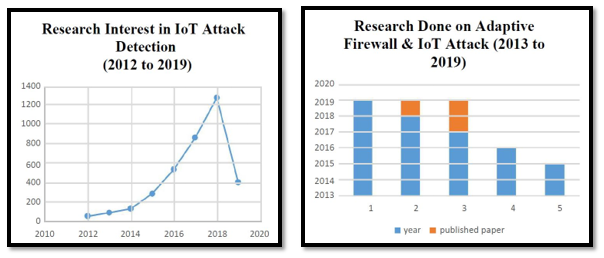
\includegraphics[scale=0.5]{Chap1/motivation.PNG}
%     \caption{Research Interest in Field of IoT}
%     \label{fig:motivation}
% \end{figure}

%  In figure \ref{fig:motivation} shows the existing research interest in IoT Attack Detection which is increasing day by day for last few years whereas for detecting attack concept of Adaptive Firewall is not so common and used term in this field. This drives us motivated to design adaptive firewall for attack detection and to block illegitimate traffic on IoT Network Model.

\section{Findings of Our Study}

Cooperative society is an association where the members voluntarily cooperate for mutual social, cultural, and economic benefit. The study reveals the following scenarios regarding how the cooperative societies in Dhaka are operating, how the members are cooperating for their mutual benefit, and how they are contributing to the socio-economic benefit of Bangladesh:

\begin{figure}[h]
    \centering
    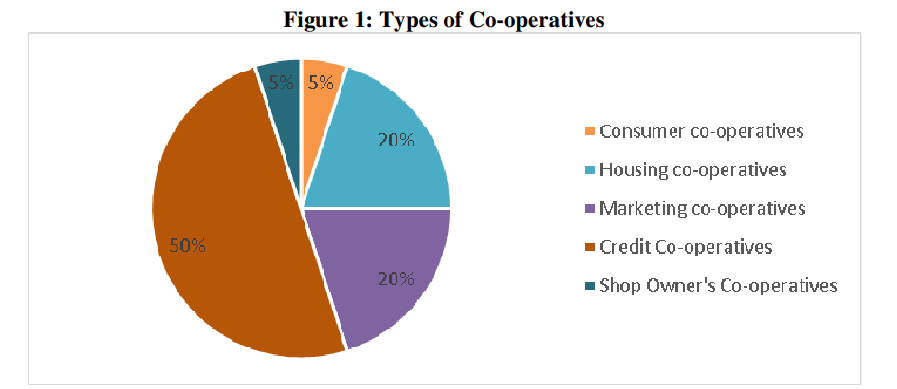
\includegraphics[width=0.6\textwidth]{Chap1/figure1.PNG}
    % \caption{Caption for your image.}
    \label{fig:example}
  \end{figure}

  Inference: Out of 20 cooperatives, Figure 1 illustrates that in Dhaka, 5\% are consumer cooperatives, 20\% are housing cooperatives, 20\% are marketing cooperatives, 50\% are credit cooperatives, and 5\% are shop owner's cooperatives.
  
  \begin{figure}[h]
    \centering
    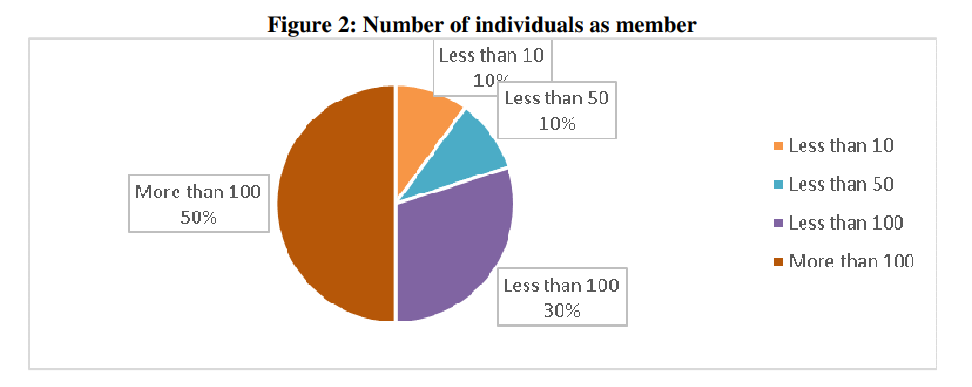
\includegraphics[width=0.6\textwidth]{Chap1/figure2.PNG}
    % \caption{Caption for your image.}
    \label{fig:example}
  \end{figure}

  Inference: Based on Figure 2, 10\% of the cooperatives out of 20 had members who are less than 10 years old. A 10\% cooperative has less than fifty members, a 30\% cooperative has less than one hundred members, and a 50\% cooperative has more than one hundred members.

\begin{figure}[h]
    \centering
    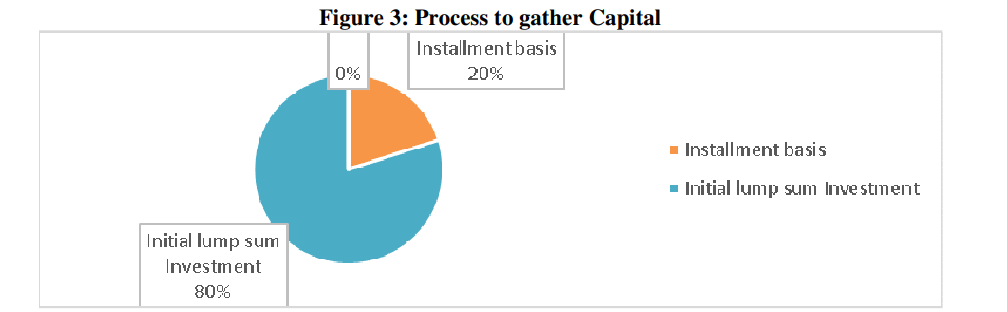
\includegraphics[width=0.6\textwidth]{Chap1/figure3.PNG}
    % \caption{Caption for your image.}
    \label{fig:example}
  \end{figure}

  Inference: The figure 3 shows that out of 20 cooperatives, 20 percent cooperatives collect their capital as 
installment basis (most of the cases monthly installment) and 80 percent cooperatives collect their capital at the 
time of launching the cooperatives as initial lump sum investment. 

\begin{figure}[h]
    \centering
    
\includegraphics[width=0.6\textwidth]{Chap1/figure4.1.PNG}
    % \caption{Registration of co-operative Societies}
    \label{fig:example}
    \centering
    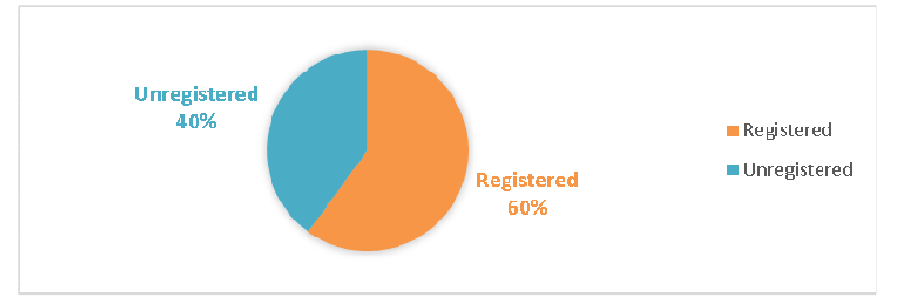
\includegraphics[width=0.6\textwidth]{Chap1/figure4.PNG}
    % \caption{Registration of co-operative Societies}
    \label{fig:example}
  \end{figure}

  Inference: The figure 4 shows that out of 20 cooperatives, 40 percent cooperatives are operating their
organization without taking registration from the concerned authority because the registration process is not easy 
due to bureaucratic problem and 60 percent co-operatives are operating by taking the registration.

\begin{figure}[h]
    \centering
    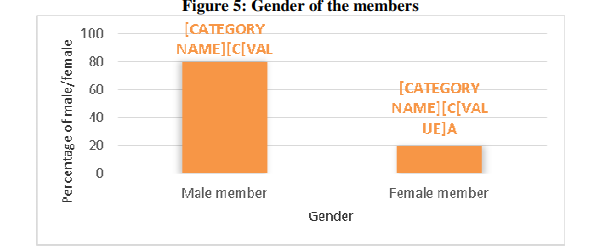
\includegraphics[width=0.6\textwidth]{Chap1/figure5.PNG}
    % \caption{Caption for your image.}
    \label{fig:example}
  \end{figure}

  Inference: The figure 5 shows that among the members in the cooperatives only 20\% members are female and 80\% members are male. So it is clear that the female participation is lower than the male participation in the cooperatives.

  \begin{figure}[h]
    \centering
    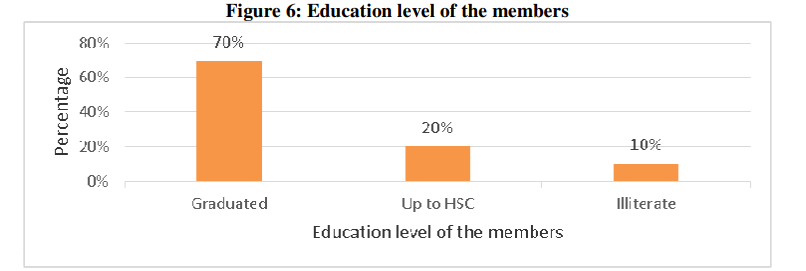
\includegraphics[width=0.6\textwidth]{Chap1/figure6.PNG}
    % \caption{Caption for your image.}
    \label{fig:example}
  \end{figure}

  Inference: The figure 6 shows that among the members in the cooperatives, 70\% are graduates, 20\% have passed up to HSC, and 10\% are illiterate.
  
  \begin{figure}[h]
    \centering
    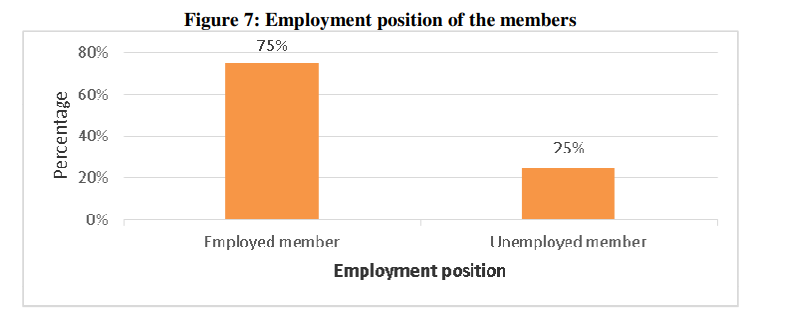
\includegraphics[width=0.6\textwidth]{Chap1/figure7.PNG}
    % \caption{Caption for your image.}
    \label{fig:example}
  \end{figure}

  Inference: The figure 7 shows that among the members in the co-operatives 75\%members are employed, 25\% members are unemployed. 

  \begin{figure}[h]
    \centering
    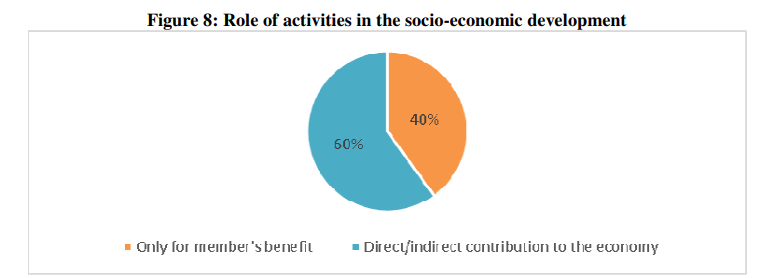
\includegraphics[width=0.6\textwidth]{Chap1/figure8.PNG}
    % \caption{Caption for your image.}
    \label{fig:example}
  \end{figure}

  Inference: The figure 8 illustrates that among the 20 cooperatives surveyed:

  \begin{itemize}
      \item 40\% of the cooperatives believe that their activities primarily benefit their members. Additionally, they express the belief that these activities may indirectly contribute to the development of the country.
      
      \item On the other hand, 60\% of the cooperatives believe that their activities directly contribute to the economic development of Bangladesh. This belief is attributed to their active participation in business-related activities.
  \end{itemize}
  

  \section{Problems of Cooperatives in Bangladesh}

The study reveals several challenges faced by cooperatives in Bangladesh:

\begin{enumerate}
    \item \textbf{Registration Challenges:}
        \begin{itemize}
            \item Many cooperatives without registration face difficulties in understanding the registration process.
            \item Bureaucratic obstacles hinder the registration process with the concerned authority.
        \end{itemize}
    
    \item \textbf{Gender Disparity:}
        \begin{itemize}
            \item Female participation in cooperatives is notably lower than male participation, impacting the true and effective realization of socio-economic benefits.
        \end{itemize}
    
    \item \textbf{Internal Conflicts:}
        \begin{itemize}
            \item Internal conflicts among cooperative members hinder progress.
            \item Predominance of vested interests within cooperatives contributes to internal conflicts.
        \end{itemize}
    
    \item \textbf{Lack of Professional Management:}
        \begin{itemize}
            \item Cooperatives suffer from a lack of professional management.
            \item Members often lack knowledge on successfully operating a cooperative.
        \end{itemize}
    
    \item \textbf{Political Interference:}
        \begin{itemize}
            \item Political interference poses a significant threat to the progress of cooperatives.
        \end{itemize}
    
    \item \textbf{Financial Constraints:}
        \begin{itemize}
            \item Limited capital supplied by members creates financial problems.
            \item Financial constraints hinder cooperatives from taking advantage of new opportunities.
        \end{itemize}
    
    \item \textbf{Lack of Motivation and Guidance:}
        \begin{itemize}
            \item Higher-level stakeholders lack motivation to highlight cooperative opportunities.
            \item Insufficient guidance is provided to obtain relative assistance from concerned authorities.
        \end{itemize}
\end{enumerate}







% \chapter{Literature Survey}
 
\chapter{Literature Review}
\label{chap:2}

\section{Related Work}

\subsection{Soft Engg}

 Several studies investigated diabetes data and constructed models to predict diabetes. Equation \ref{eq:1} give

\begin{equation} \label{eq:1}
    y=\sum_i x_i+C^2+\frac{1}{\cos{\theta}}
\end{equation}

Figure \ref{tab:sub} shows bla bla
\begin{table}[ht!]
    \centering
     \caption{Supervised Machine Learning Classifier}
     \vspace{2pt}
    \begin{tabular}{lrp{3in}}
    \hline
        \textbf{hello} & \textit{JU} & Header 2  \\ \hline
         Shamim & KMA & In this step, we will describe some supervised machine learning classifiers namedLogistic Regression, k-nearest neighbors, Support Vector Machine, Decision Tree,Gaussian Naive Bayes, Random Forest, Gradient Boosting and Linear DiscriminantAnalysis. \\  \hline
    \end{tabular}
    \label{tab:sub}
\end{table}

\section{ Machine Learning Types}

\section{Supervised Machine Learning Classifiers}

In this step, we will describe some supervised machine learning classifiers named Logistic Regression, k-nearest neighbors, Support Vector Machine, Decision Tree, Gaussian Naive Bayes, Random Forest, Gradient Boosting and Linear Discriminant Analysis. 

\subsection{Logistic Regression (LR)}

Logistic Regression (LR) is a supervised machine learning data classification algorithm that mines real-valued features from the input, multiplies each of them by a weight, adds them, and transfers the sum through a sigmoid function to produce a probability. A threshold is used to finalize a decision \cite{DSR}. A solution for classification of our data set is LR which Instead of fitting a straight line or hyperplane uses the logistic function to squeeze the output of a linear equation between 0 and 1. The logistic function is defined as:

\[Logistic (\eta) = 1/(1 + exp (-\eta))\]

As $\eta$ goes from $-\infty$ to $\infty$, logistic ($\eta$) goes from 0 to 1, a “squashing function”. In our study, we used a maximum 4000 iterations to converge the output.


\subsection{k-nearest neighbors (KNN) }
 (KNN) is a non-parametric process we used for diabetic data classification. In KNN a data is classified by a majority vote of its neighbors, with the data being allotted to the class most mutual amongst its K nearest neighbors estimated by a distance function. If K = 1, then the data is simply allotted to the class of its nearest neighbor. KNN algorithm is as below : 

\begin{algorithm}
\caption{KNN}
\label{pseudoPSO}
\begin{algorithmic}[1]
\State Let $m$ be the number of training data samples. Let $p$ be an unknown point that needs to be classified
\State Storing the training samples in an array of data points $arr[]$. Each element of this array denotes a tuple $(x, y)$.

\For{$i=0$ to $m$}
    \State Calculating distance $d(arr[i], p)$
   
\EndFor
\State Making set $S$ of $K$ smallest distances achieved. Each of these distances resembles an already classified data point
\State Returning the majority label among $S$
\end{algorithmic}
\end{algorithm}


\subsection{Decision Tree (DT)}
A DT is a classifier that recursively performs partition of the instance space. The decision tree contains nodes that form a tree, a node called “root” that has no incoming edges is the starting point of the tree. All other nodes have one incoming edge. The leaf nodes are known as decision nodes. The child node is nominated by computing Information Gain (IG).

Information Gain = Entropy(parent) - [weights average] * Entropy(children)

Entropy($Ci$) = -P($xi$) log P($xi$), where P($xi$) is the probability of child node $i$. 

Node with the highest IG will be the parent for next level. This process is continued until it gets a leaf node and completed decision tree. 

The algorithm for generating a decision tree is as below :

\begin{algorithm}
\caption{DT}
\label{pseudoPSO1}
\begin{algorithmic}[1]

\State  Create (T) 
\State Calculate frequencies (Ci, T)
\State  If all instances belong to the same class, returning leaf 
\State for every attribute a test is set for splitting criteria. An attribute that satisfies the test is test node K
\State  Repeating Create (Ti) on each partition Ti.Adding those nodes as children of node K

\end{algorithmic}
\end{algorithm}





\subsection{Gaussian Naive Bayes (GNB)}
The GNB classifier is a probability distribution function having the effect of associating neural activation to the means and variances of activation in various impulse conditions. The production of the classifier is a condition-label.  The classifier creates hypothesis that the classes have Gaussian normal distributions.

The z-score distance between the inputted point and each class-mean is estimated for each data point, namely the distance from the class mean divided by the standard deviation of that class.

\begin{equation*}
    Z_A=\frac{(x-\mu_A)}{\sigma_A}
\end{equation*}

According to the equation for a Gaussian normal distribution, each z-score is then converted into a probability value which is used for observing data point x. The co-variance between dimensions is not modelled by GNB classifier.


\subsection{Random Forest (RF)}
RF is a collective algorithm which was modelled from trees algorithm and Bagging algorithm. It works fine with a data set with a large number of input variables. It is a meta estimator that creates a number of decision tree classifiers on different sub-samples of the data set and uses mean value to increase the accuracy of the model and control over-fitting. Suppose training data set is given as: [X1, X2, X3, X4] with labels as [L1, L2, L3, L4] respectively, random forest algorithm may create three decision trees taking input of subset for example, [X1, X3, X4], [X2, X3, X4] and [X1, X2, X4]. Finally, it predicts class based on the majority of votes from each of the decision trees generated. Generally, the more trees in the forest the more robust and reliable the forest is. The random forest classifier works in the same way, the higher the number of trees in the forest gives higher accuracy output .


\subsection{Gradient boosting (GB)}
GB includes three components: a loss function that is to be optimized, a weak learner that makes predictions and an additive model which will add weak learners to minimize the loss function. 









\section{Research Gap}
Analyzing related works in this field an be noticed some shortcoming in the security measurements of IoT network. \textbf{Firstly}, there is no centralized detection method is mentioned, every layer has specific detection way method but as IoT is becoming a heterogenous network a centralized model should be proposed in controller which will control the traffic of every subpart of network. \textbf{Secondly}, by using KDD Dataset most commonly \textbf{DDoS, Probe, U2R, R2L} attack has been detected but with advancing technology intruder can attack the network in many other ways. \textbf{Thirdly}, no time efficient optimal way is mentioned to detect attack. \textbf{Fourthly}, traditional firewall can’t detect any encrypted incoming packet which can be removed by using adaptive firewall concept but still much work has not done yet regarding this problem \cite{mahmud_brain-inspired_2018,8742551,noauthor_coronavirus_nodate}.

\begin{figure}[!htb]
    \centering
    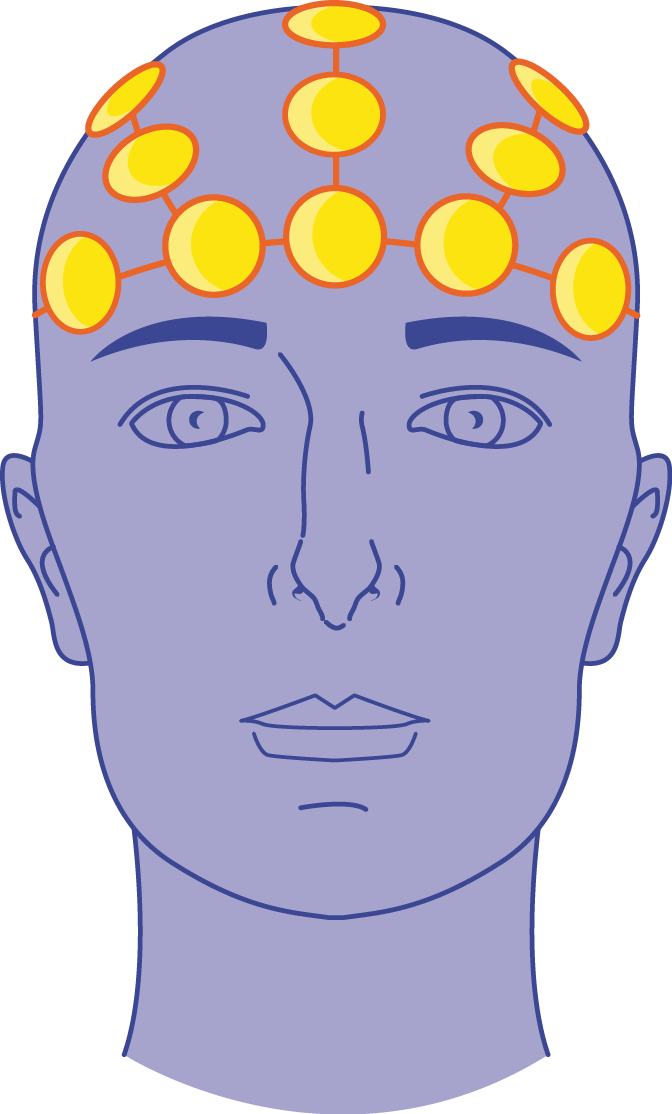
\includegraphics[scale=0.5]{Chap2/EEGonbrain.png}
    \caption{EEG probe on brain}
    \label{fig:my_label}
\end{figure}


%\chapter{System Model}
 \chapter{Design And Implementation}


\begin{figure}[h]
  \section{DATA FLOW DIAGRAM}
  \centering
  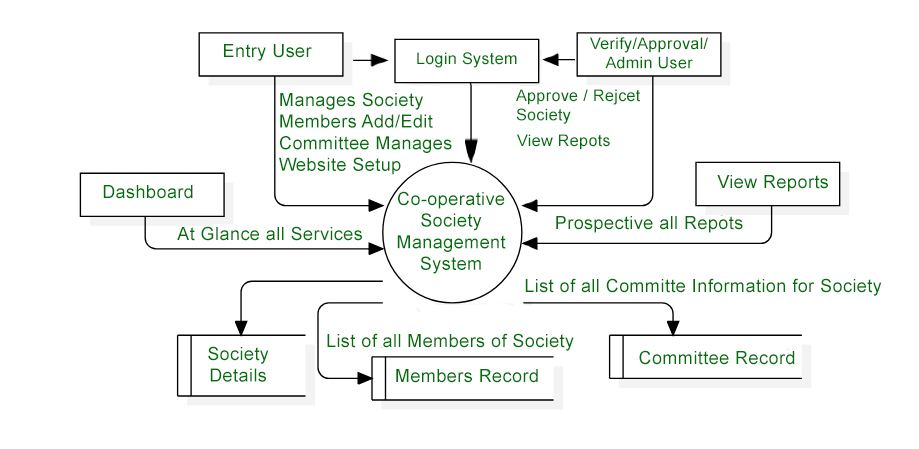
\includegraphics[width=0.6\textwidth]{Chap3/1.jpg}
  \caption{Data Flow Diagram}
  % \label{fig:example}
\end{figure}


\begin{figure}[h]
  \section{USE CASE DIAGRAM}
  \centering
  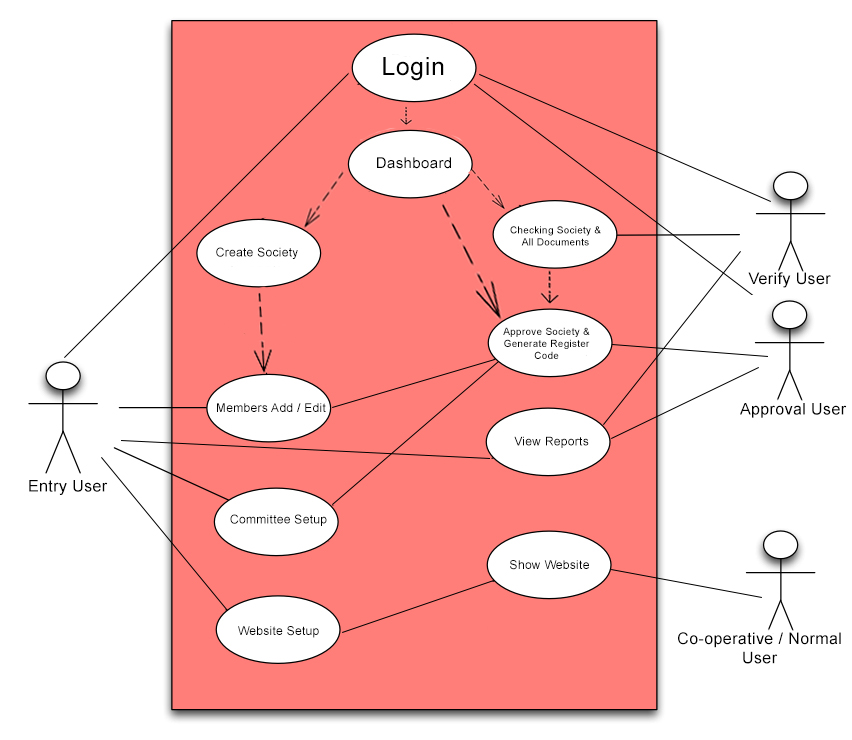
\includegraphics[width=0.6\textwidth]{Chap3/2.jpg}
  \caption{Use Case Diagram}
  \label{fig:example}
\end{figure}

\begin{figure}[h]
\section{PROCESS DIAGRAM}
  \centering
  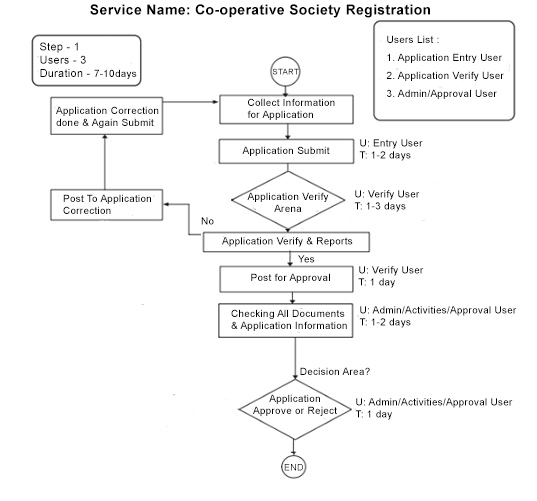
\includegraphics[width=0.6\textwidth]{Chap3/3.png}
  \caption{Process Diagram}
  \label{fig:example}
\end{figure}

\begin{figure}[h]
\section{ENTRY USER}
  \centering
  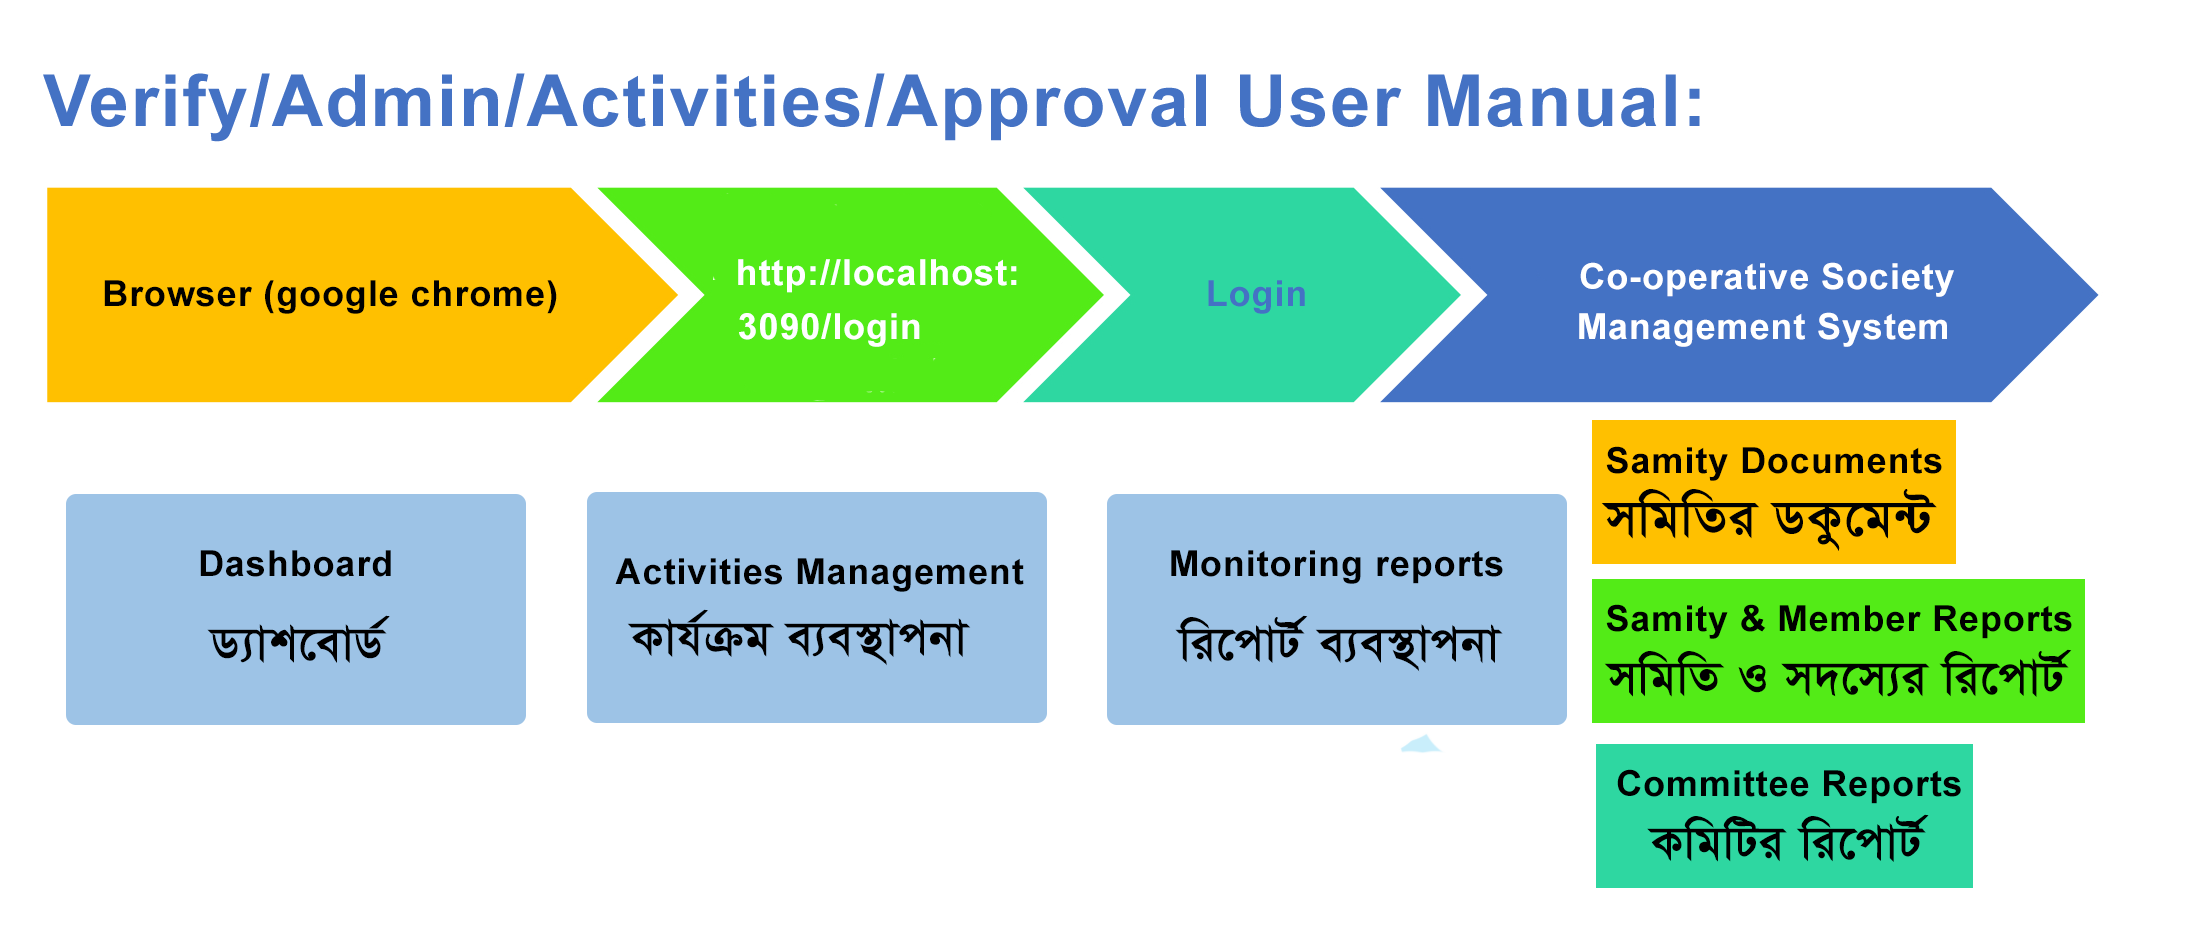
\includegraphics[width=0.6\textwidth]{Chap3/4.png}
  \caption{Entry User Diagram}
  \label{fig:example}
\end{figure}

\begin{figure}[h]
\section{VERIFY/ADMIN/ACTIVITIES/APPROVAL USER }
  \centering
  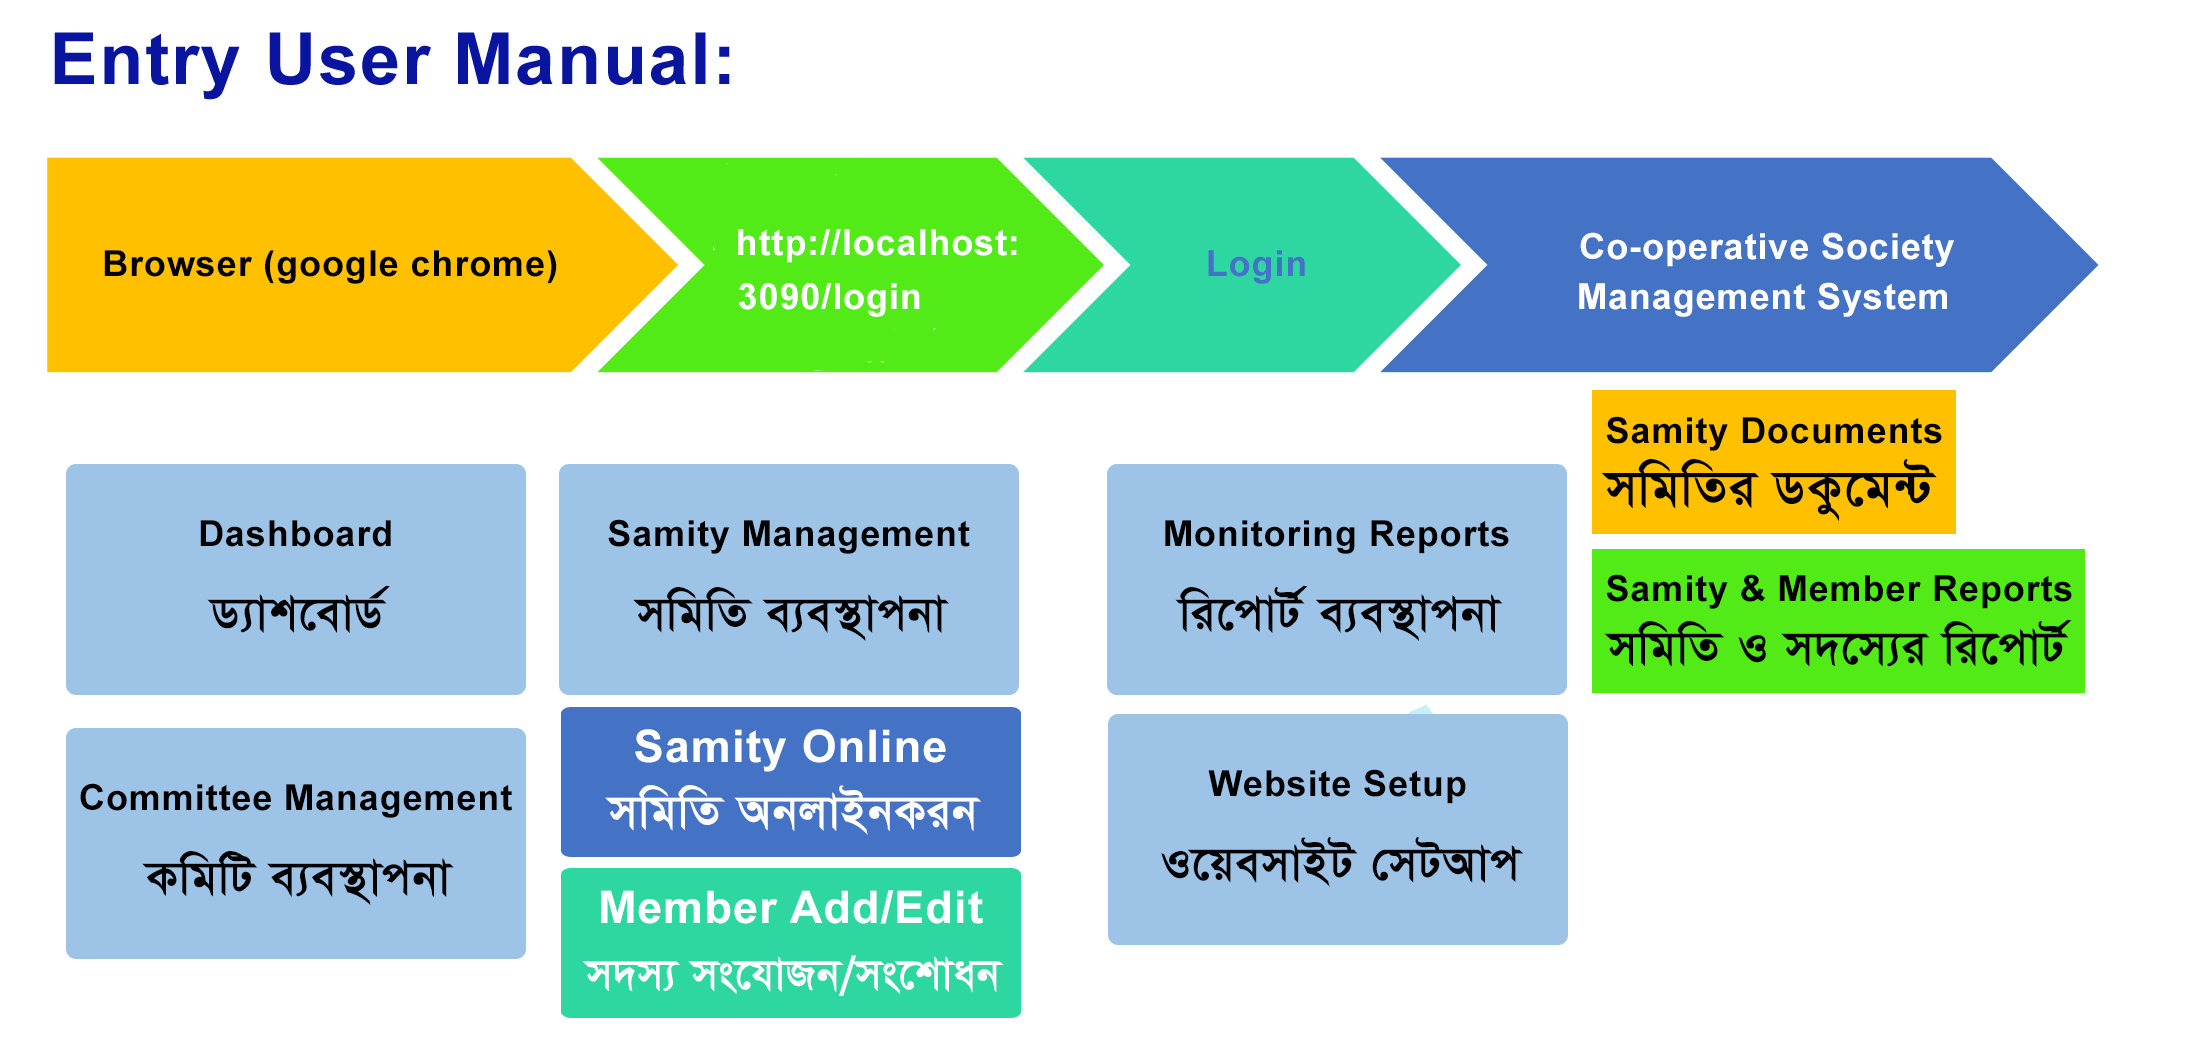
\includegraphics[width=0.6\textwidth]{Chap3/5.png}
  \caption{Verify/Admin/Activities/Approval User Diagram}
  \label{fig:example}
\end{figure}

\begin{figure}[h]
\section{RELATIONAL DATABASE DESIGN}
  \centering
  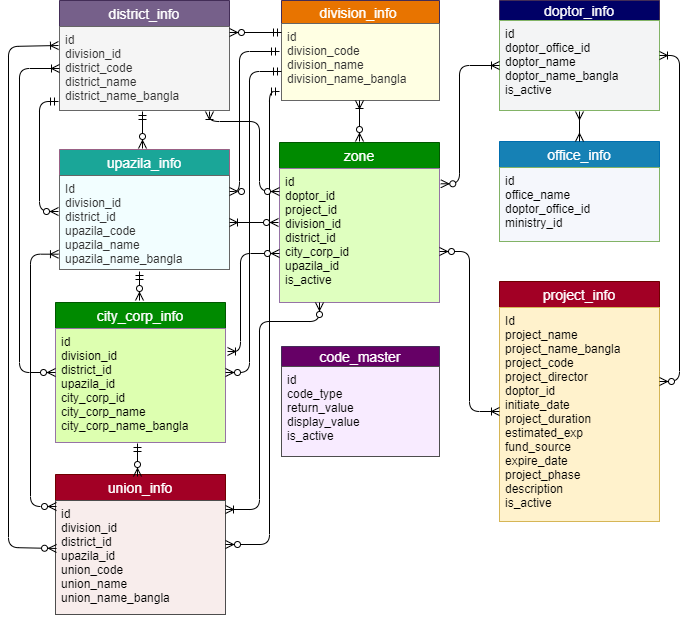
\includegraphics[width=0.6\textwidth]{Chap3/6.png}
  \caption{Zone Setup Database}
  \label{fig:example}
\end{figure}

\begin{figure}[h]
\section{SOCIETY SETUP DATABASE}
  \centering
  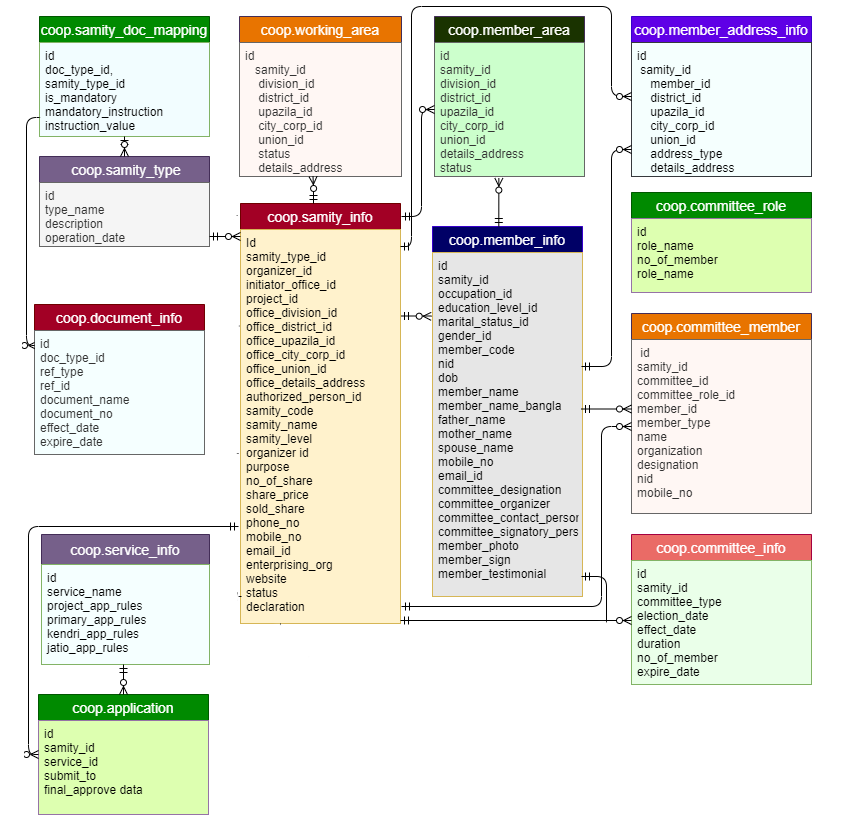
\includegraphics[width=0.6\textwidth]{Chap3/7.png}
  \caption{Society Setup Database}
  \label{fig:example}
\end{figure}

\end{document}

% ////////////////////// image sas ///////////////////////////////
\subsection{IMPLEMENTATION}

Implementing a Co-operative Society Management System involves creating a software 
application that helps manage the various activities and operations of a Co-operative society. 
Here's a basic outline of how you can implement such a system:

\subsubsection*{Dashboard:}
At a glance, show approved, rejected, pending, and waiting societies. It also displays system services based on user roles.

\subsubsection*{Society Management:}
\begin{itemize}
    \item Add and edit societies with documents in this screen by the entry user.
    \item Post to verify user follows up on his activities management and checks information and documents.
    \item Society data on the field is then submitted to the approval user.
    \item Approval user approves the society, then a 19-digit code (Example: 2023.1.01.4161.0001) is generated and stored in the society main table (\texttt{samity\_info}).
\end{itemize}

\subsubsection*{Members Management:}
\begin{itemize}
    \item Two types of entry processes: entry system and excel file upload for approved societies.
    \item Generate an ID for member code and store it in the \texttt{member\_info} table with a relational \texttt{samity\_id}.
\end{itemize}

\subsubsection*{Committee Management:}
\begin{itemize}
    \item Three types of committee types: 
    \begin{enumerate}
        \item Approved First Committee (6-12 members) with a time duration of 2 years.
        \item Elected Committee (6-12 members) with a time duration of 3 years.
        \item Election Committee (3 members) with a time duration of 90 days.
        \item Interim Committee (3 selected members) with a time duration of 45 days.
    \end{enumerate}
    \item Present committee roles as per rules. All data stored in the \texttt{committee\_info} table.
\end{itemize}

\subsubsection*{Website Setup:}
Every society gets one website for society information for Co-operative/Normal users. Set up includes Home, About Us, Members, Services, Project, and Contact of society.

\subsubsection*{Reporting:}
Generate reports on society information, member information, committee information, and overall society performance. Detailed information report attributes link to Jasper Report.





%\chapter{Simulation Results and Discussion}
\chapter{INTERFACE DESIGN}

\section{User Interface Characteristics}

Every user interface, whether designed for a Web application or a traditional software application, should exhibit the following characteristics:

\begin{itemize}
  \item \textbf{Easy to use:} The interface should be user-friendly and accessible.
  \item \textbf{Easy to learn:} Users should quickly understand how to navigate and use the system.
  \item \textbf{Easy to navigate:} Intuitive navigation enhances user experience.
  \item \textbf{Intuitive:} The interface should feel natural and be easy to understand.
  \item \textbf{Consistent:} Consistency in design elements helps users predict how the system behaves.
  \item \textbf{Efficient:} The system should allow users to accomplish tasks quickly and with minimal effort.
  \item \textbf{Error-free:} A well-designed interface minimizes the chances of user errors.
  \item \textbf{Functional:} The interface should serve its purpose effectively and meet user needs.
\end{itemize}

The Co-operative Society Management System follows all these principles of effective user interface design. Users can quickly see the breadth of their options, grasp how to achieve their goals, and do their work without being concerned with the inner workings of the system.

\section{SCREENSHOT OF THE SYSTEM}

\subsection{SYSTEM ENTRY SCREEN}
  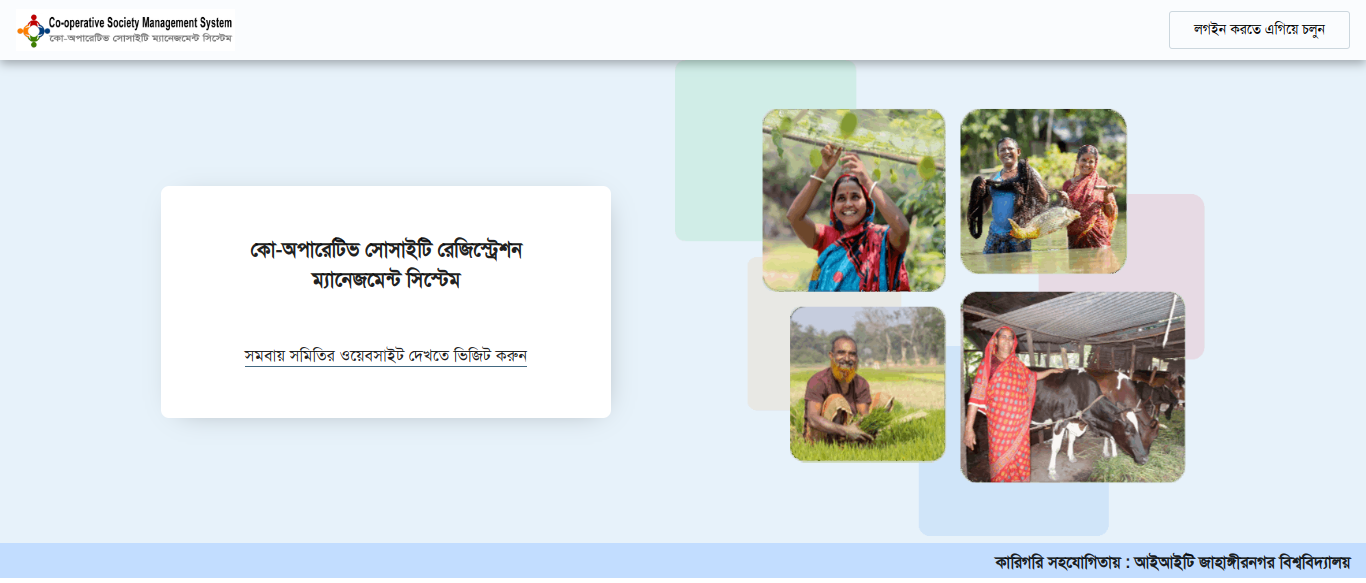
\includegraphics[width=14cm]{Chap4/1.png}

\subsection{Login Screen:}
  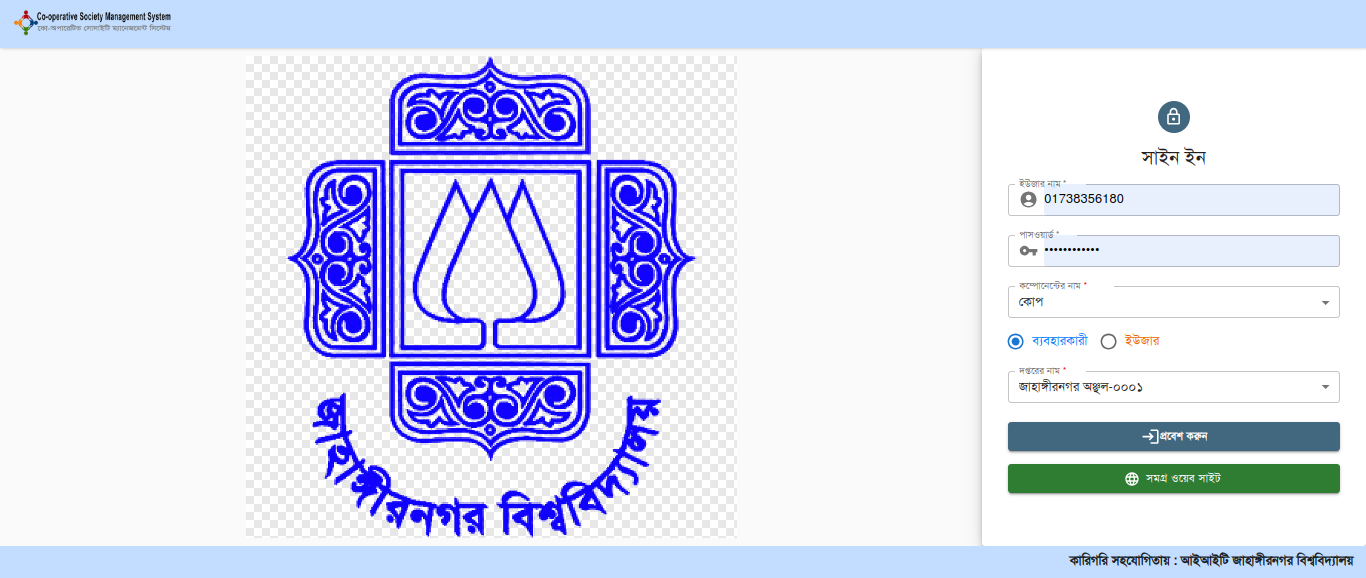
\includegraphics[width=14cm]{Chap4/2.png}
  
\subsection{User Dashboard:}
  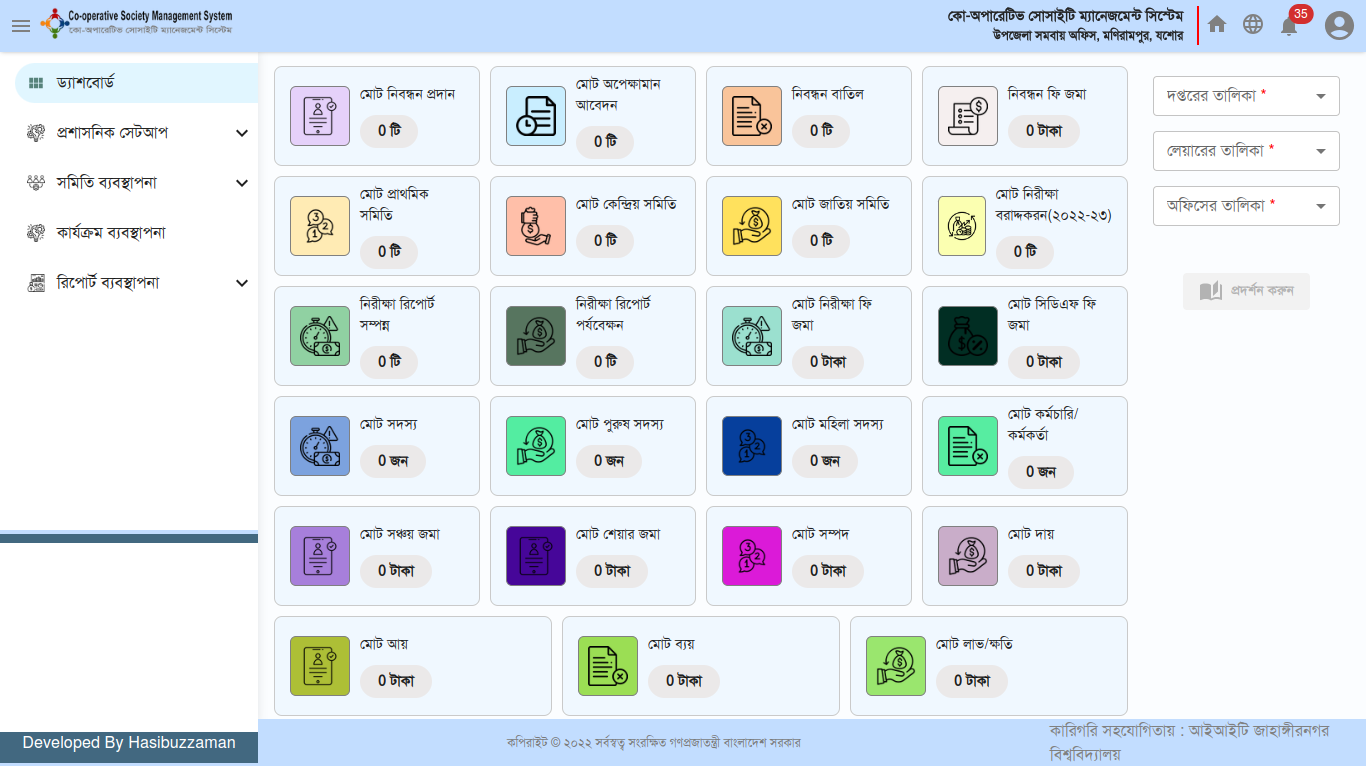
\includegraphics[width=14cm]{Chap4/3.png}

\subsection{Beneficiary Dashboard:}
  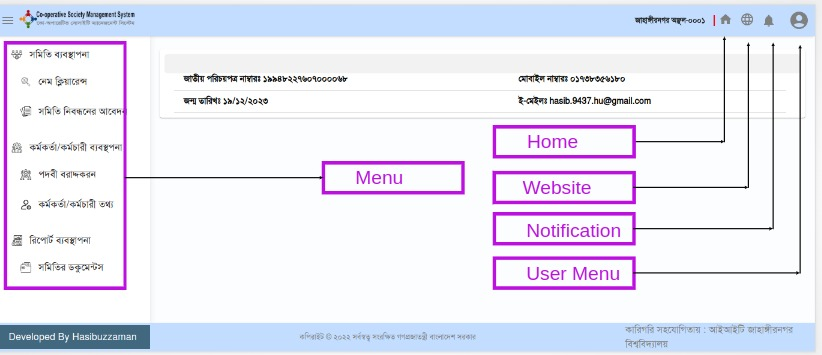
\includegraphics[width=14cm]{Chap4/4.jpeg}

\subsection{Name Clearance:}
  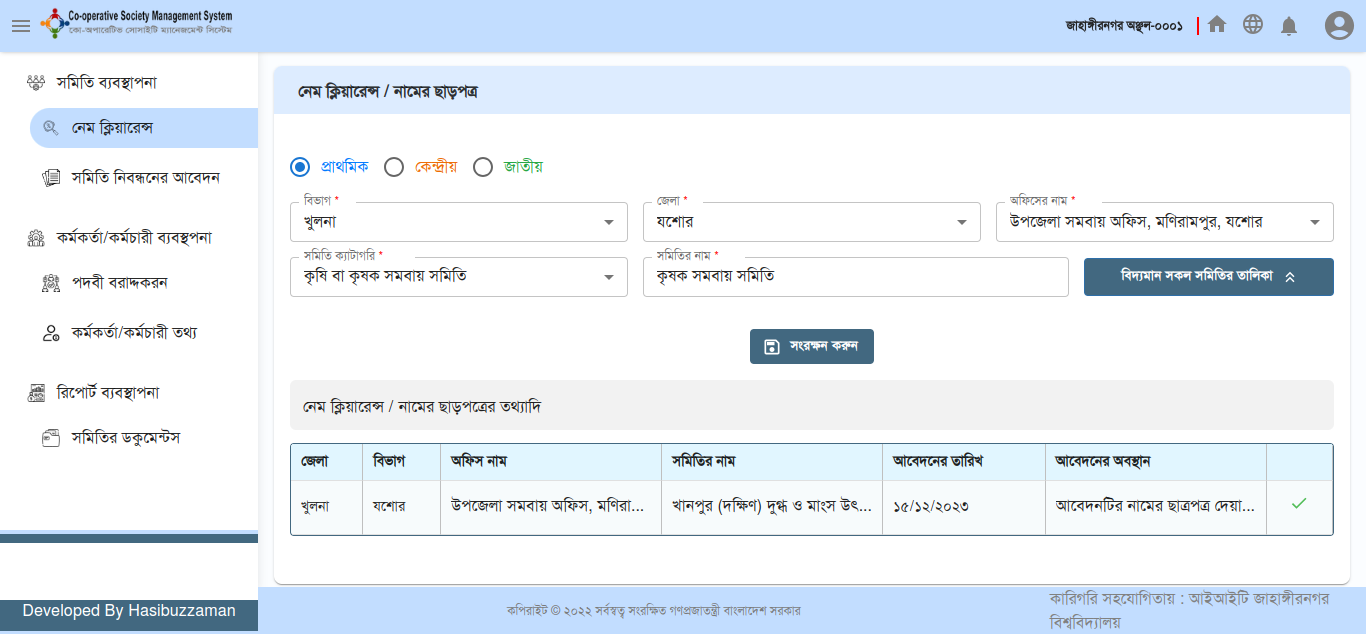
\includegraphics[width=14cm]{Chap4/5.png}

\subsection{Name Clearance:}
  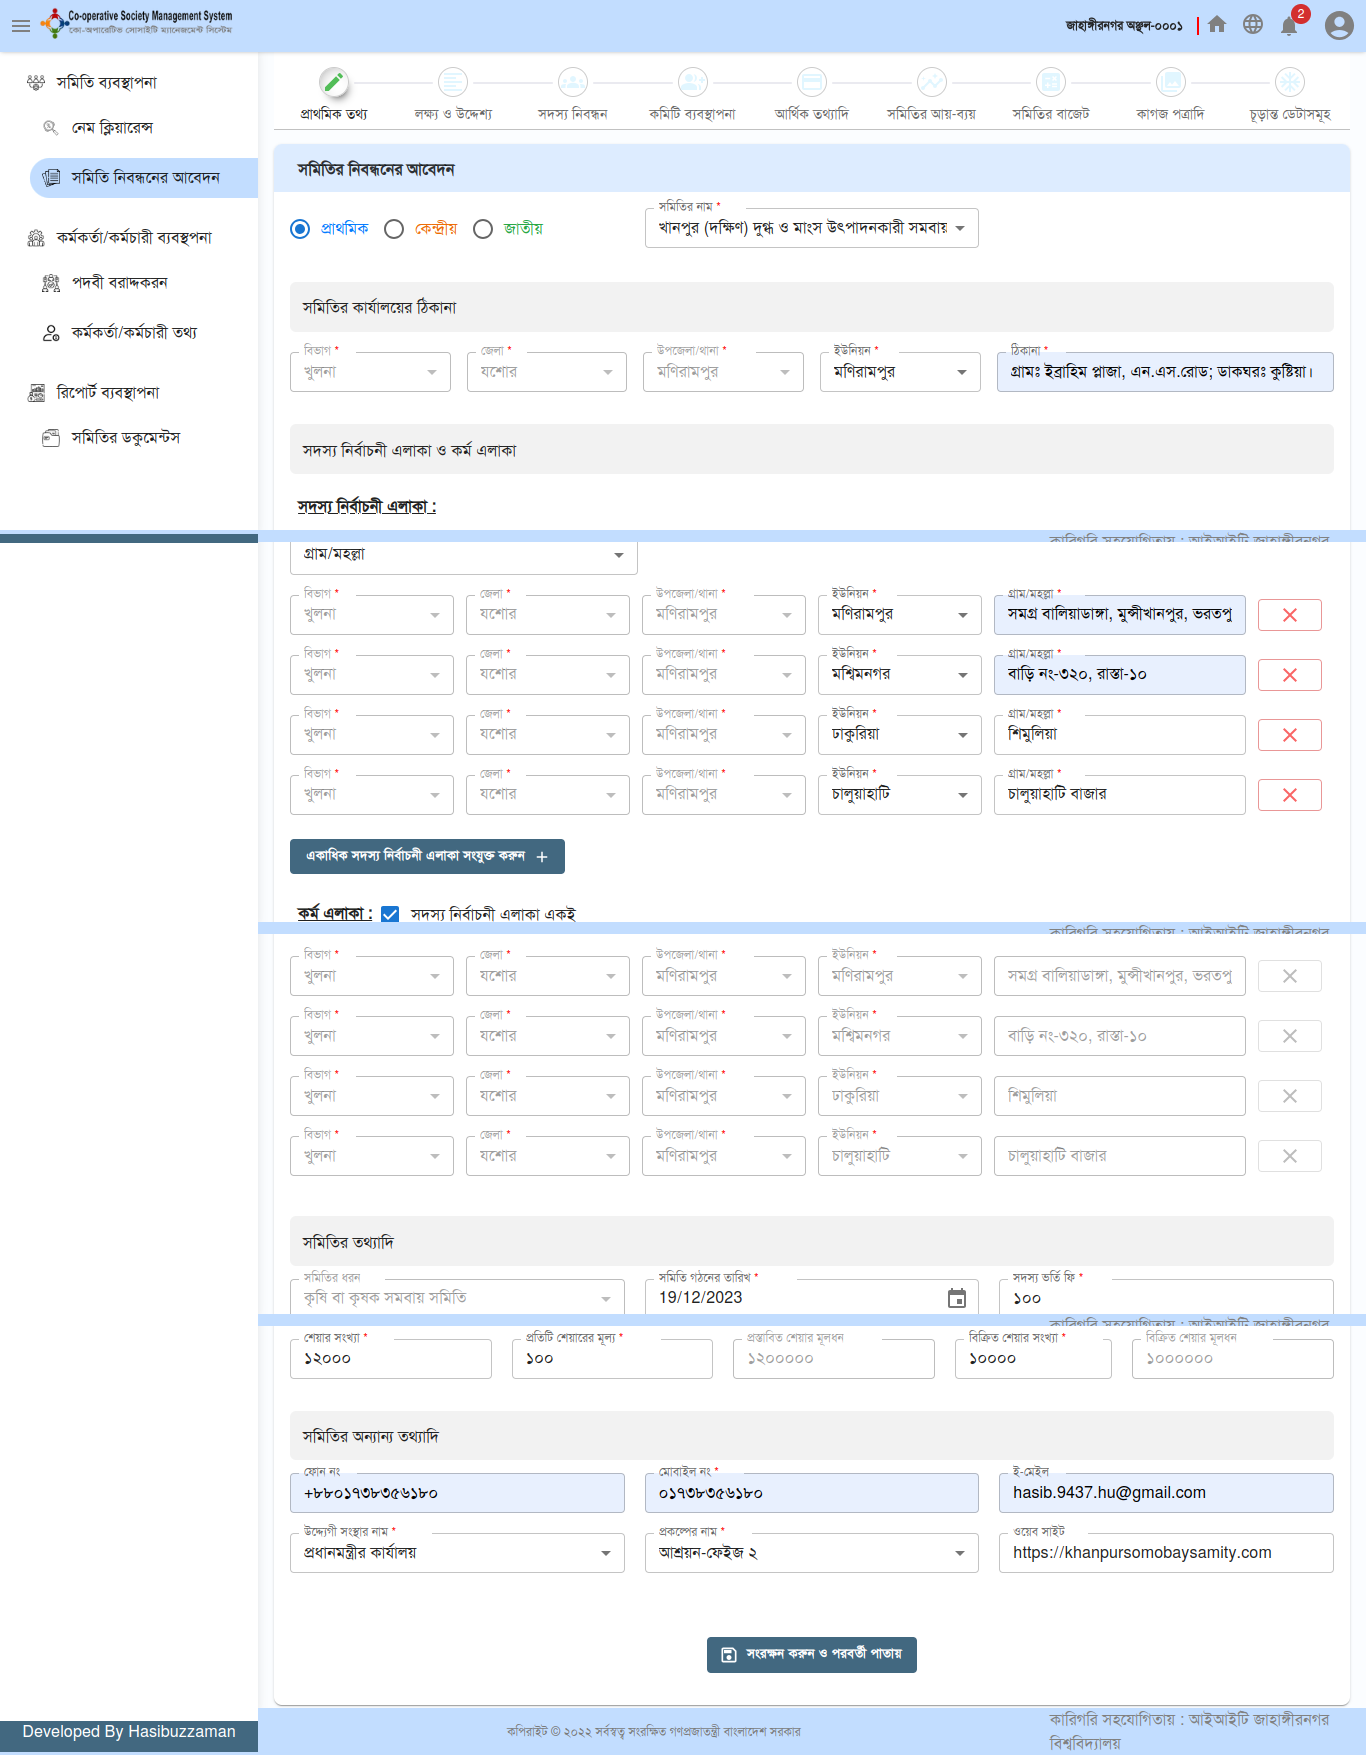
\includegraphics[width=14cm]{Chap4/6.png}

%Chapter{Performance Analysis}
\chapter{Performance Analysis}
 %This section  .... table \ref{table:2} \cite{r2}
\section{Fuzzification}
\subsection{Fuzzification Method:}
\textbf{Fuzzy logic} is a form of 
\begin{itemize}
    \item Fuzzification Unit
    \item Knowledge Based Rules
    \item Decision or Controller Unit
    \item Defuzzification Unit
\end{itemize}

%% to write equation; table and figure you have to start with \begin

\begin{equation}
    y=\cos(x)+\sin(x) +\beta
\end{equation}

where $y$ is the output of the system and $x$ is the input of the system.

\begin{figure}[ht!] %H--- must here; h-- here, t--top, b--bottom
    \centering
    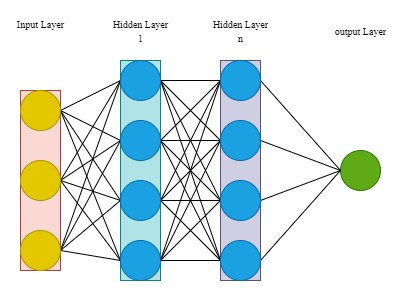
\includegraphics[scale=0.5]{Chap5/cnn1.jpg}
    \caption{CNN architecture}
    \label{fig:CNN}
\end{figure}


Figure \ref{fig:CNN} shows a CNN architecture. 


\begin{table}[]
    \centering
    \caption{Deep learning Algorithms \cite{mondal_automatic_2017}}
    \begin{tabular}{cp{2in}} %c--center, l--left, r--right; p-- width
      \hline %horizontal line
      \textbf{Name of Algorithm}   & \textbf{Description}  \\ \hline
        CNN & It includes input, hidden and output layers .\\ \hline
        RNN & It is useful for time series data. It takes output and fed into input \\ \hline
    \end{tabular}
        \label{tab:DL}
\end{table}

Table  \ref{tab:DL}     shows deep learning algorithm \cite{wiki_2016}.





%\chapter{Conclusion and Future Work}
\chapter{Discussion and Conclusion}



\section{Limitations}
Co-operative society management systems, like any other systems, have their limitations. Here
are some common limitations associated with Co-operative society management systems:

a. Limited Resources

b. Technical Expertise

c. Data Security Concerns

d. Integration Challenges

e. Limited Access to Technology

f. Resistance to Change

g. Maintenance and Upkeep

h. Customization Needs

i. Dependency on Vendors

j. Legal and Regulatory Compliance 

Addressing these limitations requires careful planning, adequate resources, and a willingness to
adapt to new technologies and processes. Co-operative societies need to assess their unique
needs and challenges to select and implement a management system that aligns with their
objectives and resources.

\section{Future Plan}
Creating a robust Co-operative society management system requires careful planning and
consideration of various aspects. Here's a future-oriented plan to enhance the efficiency and
effectiveness of a Co-operative society management system:

a. Digital Transformation

b. Data Security and Privacy

c. Member Engagement:

d. Financial Management:

e. Governance and Compliance

f. Community Building

g. Analytics and Reporting:

h. Continuous Improvement

i Disaster Preparedness

j. Environmental Sustainability

By integrating these strategies, a Co-operative society can not only streamline its operations but
also enhance member satisfaction, foster community engagement, and ensure long-term
sustainability in an ever-changing future landscape. 

\section{Conclusion}

The implementation of a Co-operative Society Management System can have several positive outcomes for both the society and its members.

In conclusion, a Co-operative Society Management System not only modernizes the functioning of the society but also enhances member satisfaction, financial stability, and community development. It is a strategic investment that can pave the way for the sustainable growth of Cooperative societies in the future.
% \label{chap:conclusion}
% \chapter{Performance Analysis}
 %This section  .... table \ref{table:2} \cite{r2}
\section{Fuzzification}
\subsection{Fuzzification Method:}
\textbf{Fuzzy logic} is a form of 
\begin{itemize}
    \item Fuzzification Unit
    \item Knowledge Based Rules
    \item Decision or Controller Unit
    \item Defuzzification Unit
\end{itemize}

%% to write equation; table and figure you have to start with \begin

\begin{equation}
    y=\cos(x)+\sin(x) +\beta
\end{equation}

where $y$ is the output of the system and $x$ is the input of the system.

\begin{figure}[ht!] %H--- must here; h-- here, t--top, b--bottom
    \centering
    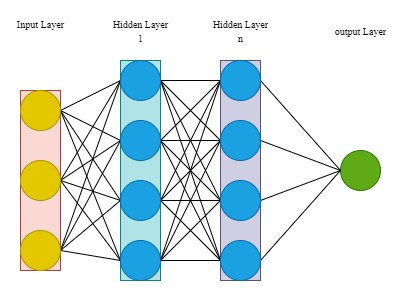
\includegraphics[scale=0.5]{Chap5/cnn1.jpg}
    \caption{CNN architecture}
    \label{fig:CNN}
\end{figure}


Figure \ref{fig:CNN} shows a CNN architecture. 


\begin{table}[]
    \centering
    \caption{Deep learning Algorithms \cite{mondal_automatic_2017}}
    \begin{tabular}{cp{2in}} %c--center, l--left, r--right; p-- width
      \hline %horizontal line
      \textbf{Name of Algorithm}   & \textbf{Description}  \\ \hline
        CNN & It includes input, hidden and output layers .\\ \hline
        RNN & It is useful for time series data. It takes output and fed into input \\ \hline
    \end{tabular}
        \label{tab:DL}
\end{table}

Table  \ref{tab:DL}     shows deep learning algorithm \cite{wiki_2016}.




%\startbibliography
 %\begin{singlespace} % Bibliography must be single spaced
%\bibliography{References}   % Use the BibTeX file ``References.bib''.
%\end{singlespace}
%%\setlinespacing{1.44}
\bibliographystyle{ieeetr}
%\bibliography{xbib}
% An external Abstract that can be printed at the end of the document,
% for separate submission to Rackham. Comment it out when not needed. - jg
%\startextabstractpage
%{The Title of Your Dissertation}{Your Name}{Chair: Albert Einstein}
%The Co-operative Society Management System is a comprehensive software solution created to streamline and automate the functions of Co-operative societies under the Bangladesh Rural Development Co-operative Division authority. This summary offers insights into its main features and advantages.

Co-operative societies are pivotal in sectors like agriculture, finance, and housing, fostering collaboration among members and fostering economic development. Yet, the management of administrative tasks and financial transactions within these societies can be intricate and time-intensive. The Co-operative Society Management System seeks to simplify these processes by providing an efficient and user-friendly platform.






\vspace{8pt}
\textbf{Keywords:} Coop, Co-operative Society Management System, Socity Management System, cooperative and loan Management System and Samity Management System.

%\label{ExtAbstract}

%\bibliographystyle{alpha}
%\bibliographystyle{alpha}

% \bibliography{bibfile}

\end{document}
